\setcounter{chapter}{1}
\chapter{Le langage Assembleur}

\section*{Introduction}

Dans ce chapitre, il faut rendre les exercices 2.2, 2.3, 2.9 et un exercice au choix. L'exercice 2.10 est un bonus pour les plus audacieux.

\section{Exercice 2.2 (A rendre)}

\subsection{Question}
Écrivez en assembleur une fonction delta() qui renvoie b\textsuperscript{2} − 4ac calculée avec quatre variables globales a, b, c et delta. Expliquez.

N'oubliez pas d'écrire également le programme C appelant et d'insérer les copies d'écran (ou textuelles) commentées avec deux ou trois exemples distincts.

\subsection{Développement}
Pour mener à bien cet exercice, nous avons adopté le processus suivant :

Le but est de calculer le discriminant d'une équation du second degré : $\Delta = b^2 - 4ac$.
Pour ce faire, nous utilisons une architecture \textbf{x86 32 bits}. L'interaction entre le langage C et l'Assembleur se fait via des \textbf{variables globales}.

\begin{itemize}
    \item \textbf{Le programme C} : Il déclare les variables en mémoire vive, leur assigne des valeurs et appelle la fonction assembleur.
    \item \textbf{Le programme Assembleur} : Il récupère les valeurs depuis la mémoire, effectue les calculs dans les registres du processeur (\texttt{\%eax}, \texttt{\%ebx}), puis écrit le résultat final dans la variable \texttt{delta}.
\end{itemize}

\begin{enumerate}
    \item \textbf{Création des sources :} Rédaction des fichiers \texttt{main.c} et \texttt{delta.s} avec les métadonnées et commentaires requis.
\end{enumerate}

\subsubsection*{Fichier Assembleur (\texttt{delta.s})}

\begin{figure}[htbp]
    \centering
    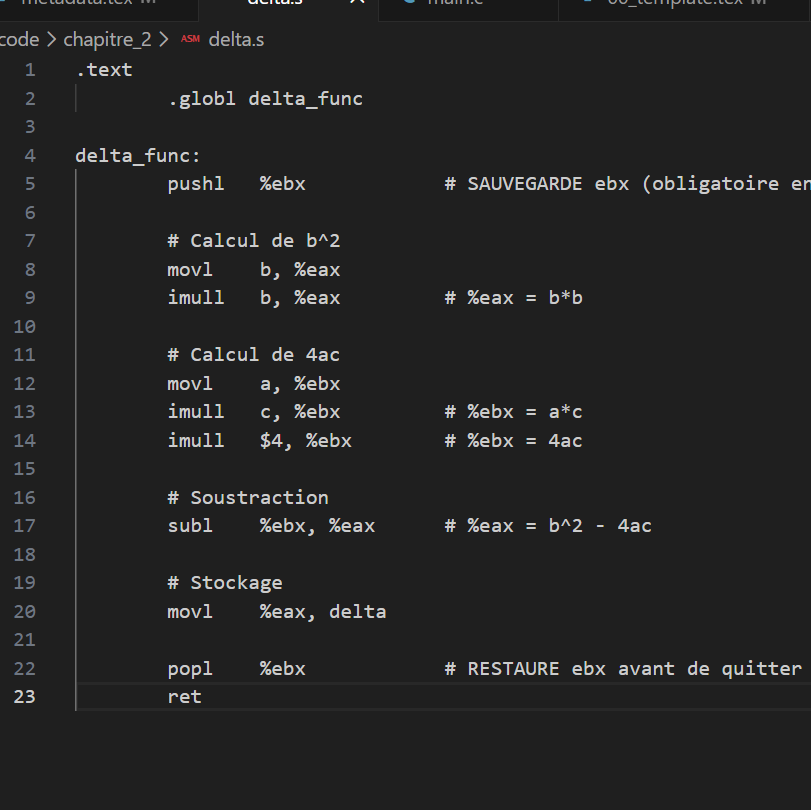
\includegraphics[width=0.85\textwidth]{images/fichier_assembleur.png} 
    \caption{Extrait du code source de delta.s commenté}
    \label{fig:code_delta}
\end{figure}

Nous utilisons la syntaxe \textbf{AT\&T}. Notez l'utilisation de \texttt{pushl} et \texttt{popl} pour protéger le registre \texttt{\%ebx}, garantissant la stabilité du programme.

\begin{figure}[htbp]
    \centering
    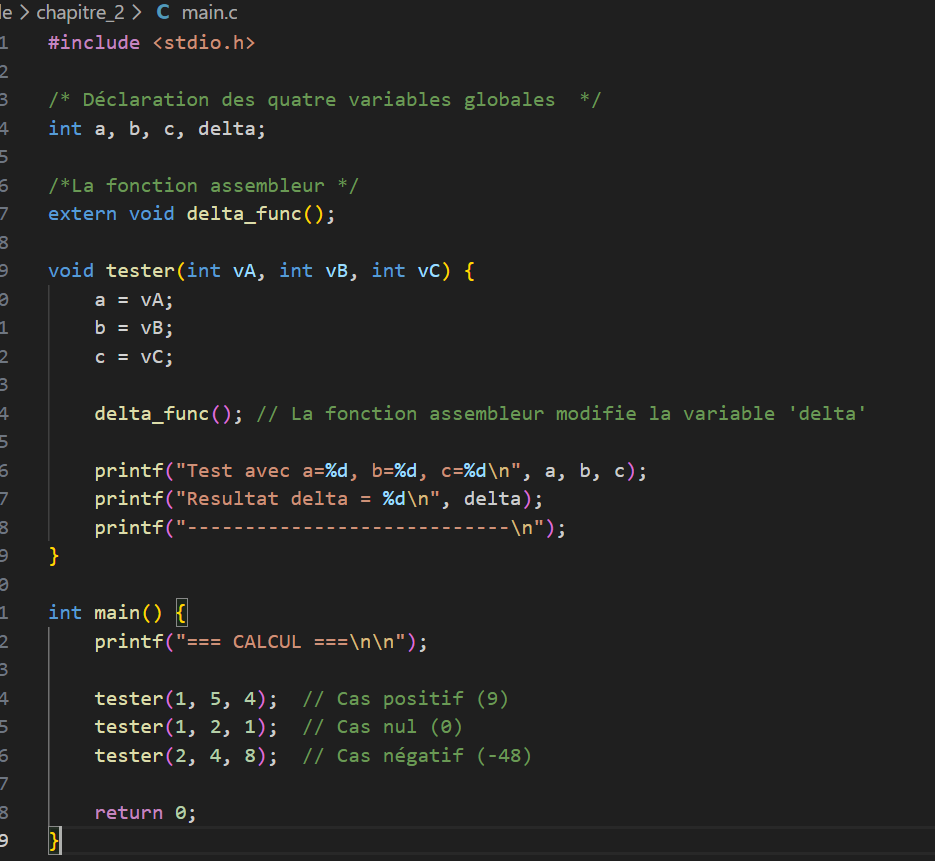
\includegraphics[width=0.85\textwidth]{images/fichier_main.png} 
    \caption{Extrait du code source de main.c commenté}
    \label{fig:code_main}
\end{figure}

\subsubsection*{Compilation et exécution}

\noindent\textit{Note :} Pour compiler sur un système moderne (comme Kali Linux), nous devons forcer le mode 32 bits et autoriser l'accès aux variables globales simples.

\begin{figure}[htbp]
    \centering
    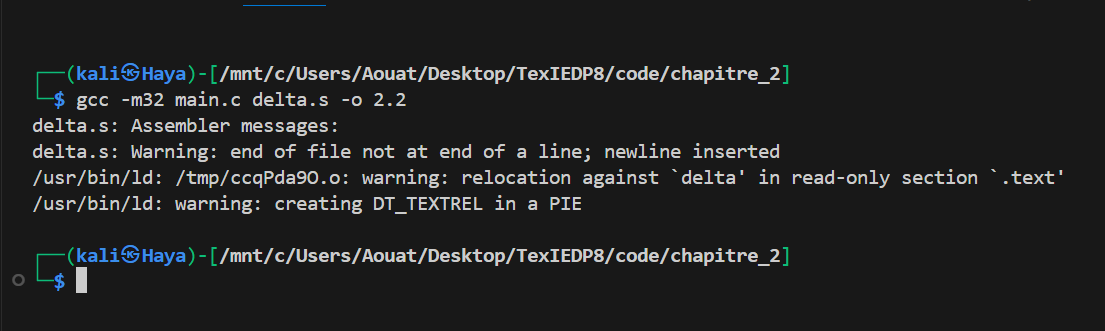
\includegraphics[width=0.85\textwidth]{images/cmd2_2.png} 
    \caption{Commande de compilation et exécution}
    \label{fig:cmd_compile}
\end{figure}

\noindent\textit{Commentaires :} Il manquait une ligne à la fin de mon fichier \texttt{delta.s}. J'ai donc rajouté \texttt{.end}. Pour enlever l'avertissement \texttt{DT\_TEXTREL}, j'ai rajouté une option à ma commande :

\begin{verbatim}
gcc -m32 -no-pie main.c delta.s -o 2.2
./2.2
\end{verbatim}

\subsubsection*{Réponse et analyse des résultats}

Voici la capture textuelle du résultat après exécution du programme :

\begin{figure}[htbp]
    \centering
    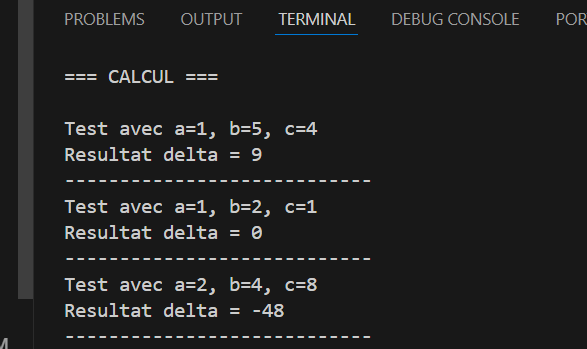
\includegraphics[width=0.85\textwidth]{images/res2_2.png} 
    \caption{Résultat de l'exécution du programme}
    \label{fig:resultat_exec}
\end{figure}

\paragraph*{Interprétation :}

\begin{itemize}
    \item \textbf{Exemple 1 ($\Delta = 9$)} : Le résultat est positif. Mathématiquement, cela signifie que l'équation possède \textbf{deux racines réelles} distinctes.
    \item \textbf{Exemple 2 ($\Delta = 0$)} : Le résultat est nul. Cela signifie que l'équation possède \textbf{une racine double} (le sommet de la parabole touche l'axe des abscisses).
    \item \textbf{Exemple 3 ($\Delta = -48$)} : Le résultat est négatif. L'équation ne possède \textbf{aucune racine réelle}.
\end{itemize}

\section{Exercice 2.3 (A rendre)}
\subsection{Question}
Écrivez en assembleur une fonction médian3 qui reçoit trois arguments et renvoie celui qui n'est ni le plus grand, ni le plus petit.

\textbf{Remarque :} La fonction est utile dans Quick Sort pour choisir le pivot entre le premier élément, le dernier et celui du milieu.

\textbf{Note :} N'oubliez pas d'écrire également le programme C appelant et d'insérer les copies d'écran (ou textuelles) commentées avec deux ou trois exemples distincts.

\subsection{Développement}
La fonction median3 a pour but d'extraire la valeur centrale parmi trois entiers ($a$, $b$, et $c$). Contrairement à un tri complet qui nécessiterait d'ordonner les trois éléments, trouver la médiane ne demande que quelques comparaisons logiques.

En algorithmique, on utilise un arbre de décision. L'idée est la suivante : on compare $a$ et $b$. Selon le résultat, on compare le troisième élément ($c$) avec les deux autres pour situer lequel est "au milieu".

Cette méthode est cruciale dans l'algorithme Quick Sort : choisir la médiane comme "pivot" permet d'éviter les pires cas de performance (complexité $O(n^2)$) lorsque le tableau est déjà presque trié.

Les arguments arrivent dans les registres \texttt{\%rdi}, \texttt{\%rsi}, et \texttt{\%rdx}. Le résultat est renvoyé dans \texttt{\%rax}.

\subsubsection*{Code source}

\begin{figure}[htbp]
    \centering
    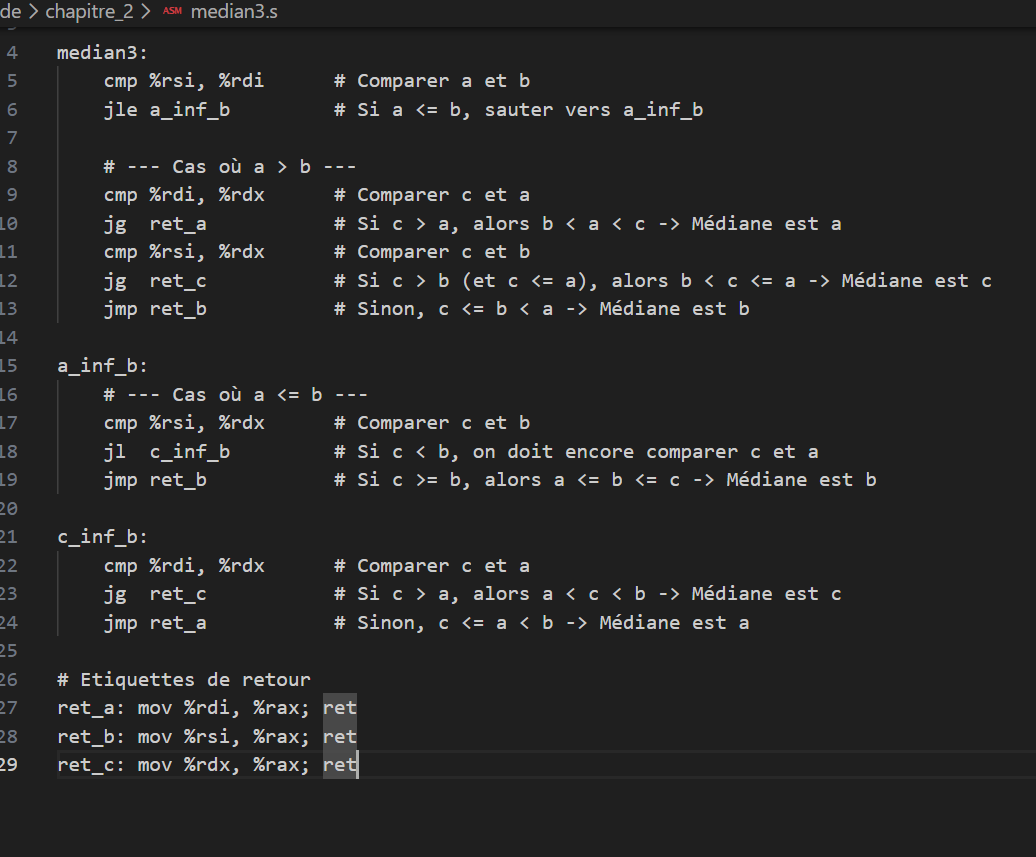
\includegraphics[width=0.85\textwidth]{images/median3_assembleur.png} 
    \caption{Nous utilisons la syntaxe AT\&T. Le résultat est renvoyé dans \texttt{\%rax}}
    \label{fig:code_median3_assembleur}
\end{figure}

\begin{figure}[htbp]
    \centering
    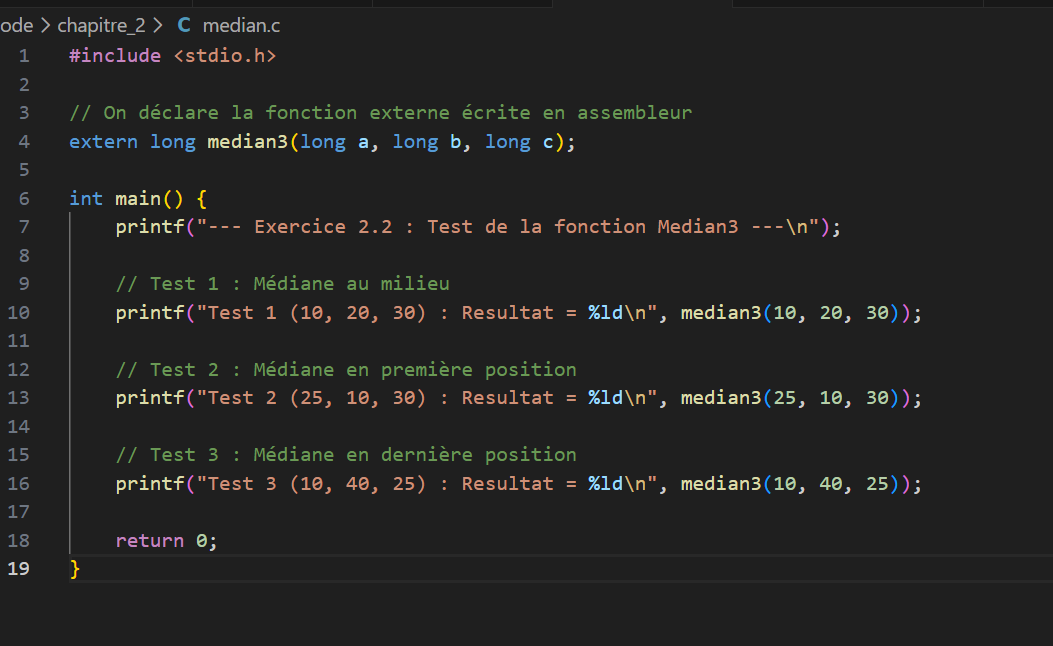
\includegraphics[width=0.85\textwidth]{images/median3_c.png} 
    \caption{Extrait du code source de main.c commenté. Ce fichier permet de tester la fonction avec différents scénarios}
    \label{fig:code_main_median3_c}
\end{figure}

\subsubsection*{Compilation et exécution}   

Pour compiler et exécuter le programme, nous utilisons les commandes suivantes :

\begin{verbatim}
gcc -o exo2.3 median.c median3.s
./exo2.3
\end{verbatim}

\begin{figure}[htbp]
    \centering
    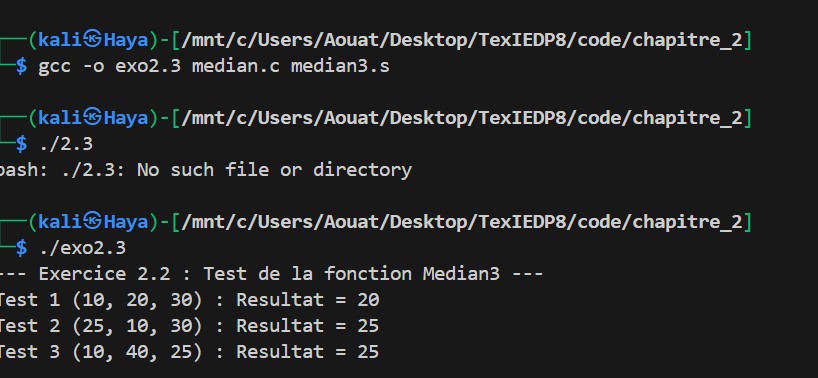
\includegraphics[width=0.85\textwidth]{images/res2_3.png} 
    \caption{Résultat de l'exécution du programme}
    \label{fig:resultat_exec_median3}
\end{figure}

\subsubsection*{Réponse et analyse des résultats}

\paragraph*{Interprétation :}

\begin{itemize}
    \item \textbf{Exemple 1 (Médiane = 20)} : Les valeurs $10$, $20$, et $30$ sont fournies. La médiane correcte est $20$.
    \item \textbf{Exemple 2 (Médiane = 25)} : Les valeurs $25$, $10$, et $30$ sont fournies. La médiane correcte est $25$.
    \item \textbf{Exemple 3 (Médiane = 25)} : Les valeurs $10$, $40$, et $25$ sont fournies. La médiane correcte est $25$.
\end{itemize}

L'implémentation est efficace car elle n'utilise que les registres processeurs, évitant ainsi les accès lents à la mémoire RAM. Le passage par les étiquettes (labels) permet de ne réaliser que 2 à 3 comparaisons au maximum par appel, ce qui est optimal pour une intégration dans un algorithme de tri haute performance comme Quick Sort.

\section{Exercice 2.4 (Au choix mais à rendre)}

\subsection{Question}
Écrivez en assembleur une fonction \texttt{myStrLen} équivalente à la fonction C \texttt{strlen()}.

\textbf{Rappel :} pour n'accéder qu'à un seul octet, il faut postfixer l'instruction avec \texttt{b} (byte) au lieu de \texttt{l} (long). Vous aurez à utiliser \texttt{cmpb}.

\subsection{Développement}
\texttt{cmpb \$0, (\%edx)} : C'est l'instruction clé. \texttt{cmpb} signifie "compare byte" (comparer un octet). On regarde si le caractère actuel est le zéro binaire qui termine toutes les chaînes en C.

\texttt{incl \%eax} : Chaque fois qu'on trouve un caractère qui n'est pas zéro, on ajoute 1 à notre compteur.

\texttt{incl \%edx} : On avance le pointeur dans la mémoire pour lire le caractère suivant.

Le résultat : En C, par convention, la valeur de retour d'une fonction doit toujours se trouver dans le registre \texttt{\%eax}. C'est pour cela qu'on utilise \texttt{\%eax} comme compteur.

\subsubsection*{Code source}

\begin{figure}[htbp]
    \centering
    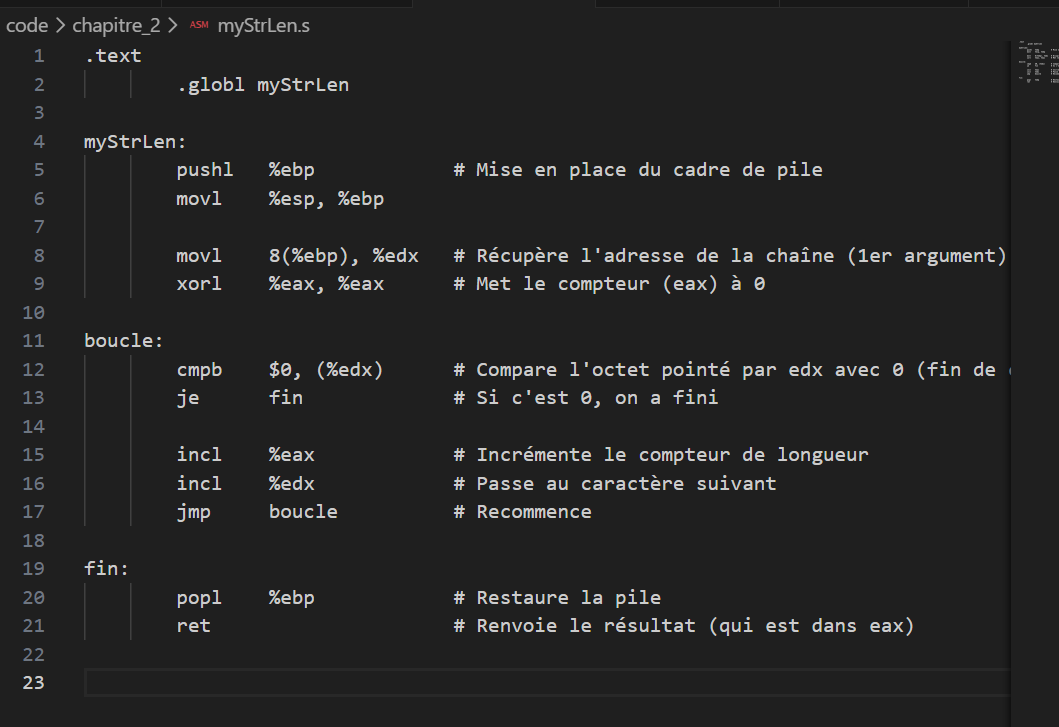
\includegraphics[width=0.85\textwidth]{images/mystrlen_assem.png} 
    \caption{Extrait du code source de myStrLen.s commenté}
    \label{fig:code_mystrlen_assembleur}
\end{figure}

\begin{figure}[htbp]
    \centering
    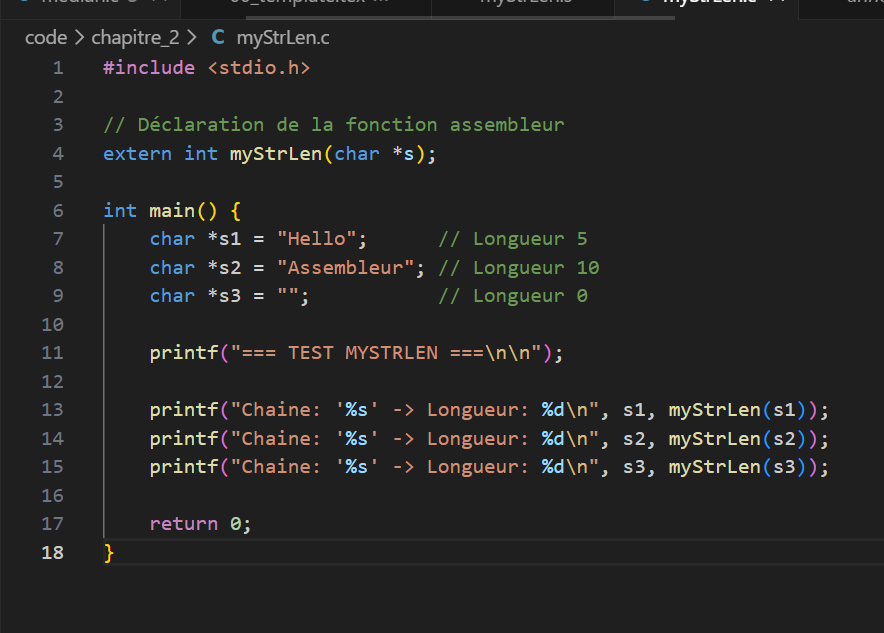
\includegraphics[width=0.85\textwidth]{images/mystrlen_c.png} 
    \caption{Extrait du code source de main.c commenté. Ce fichier permet de tester la fonction avec différents scénarios}
    \label{fig:code_main_mystrlen_c}
\end{figure}

\subsubsection*{Compilation et exécution}

On utilise les mêmes commandes que tout à l'heure pour compiler et exécuter le programme :
\begin{verbatim}
gcc -m32 -o exo2.4 myStrLen.c myStrLen.s
./exo2.4
\end{verbatim}

\begin{figure}[htbp]
    \centering
    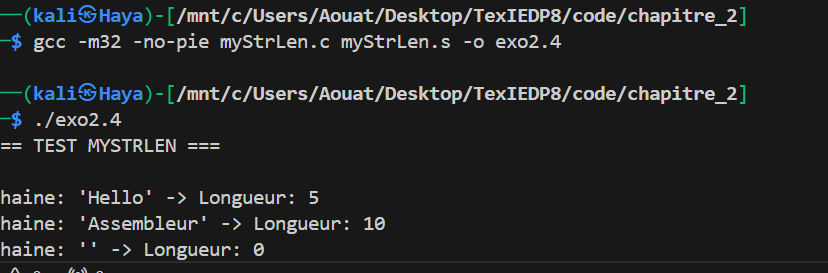
\includegraphics[width=0.85\textwidth]{images/res2_4.png} 
    \caption{Commande de compilation et exécution}
    \label{fig:cmd_compile_mystrlen}
\end{figure}

\subsubsection*{Réponse et analyse des résultats}

L'implémentation de \texttt{myStrLen} illustre la communication directe entre le processeur et la mémoire :

\textbf{Parcours Mémoire :} La fonction traite une chaîne comme une succession d'octets. Le registre \texttt{\%edx} sert de pointeur mobile jusqu'à la rencontre du caractère nul (\textbackslash0).

\textbf{Précision Chirurgicale (\texttt{cmpb}) :} L'usage de \texttt{cmpb} montre comment l'assembleur manipule les données à l'échelle de l'octet, l'unité de base du type \texttt{char}.

\textbf{Lien C/Assembleur :} L'utilisation de \texttt{\%eax} pour stocker le compteur final respecte la convention d'appel x86, permettant au programme C de récupérer automatiquement la longueur calculée.

Cet exercice démontre qu'une fonction simple en C repose sur une gestion rigoureuse des registres et de la pile en assembleur pour garantir la stabilité du système.
\section{Exercice 2.9 (A rendre)}

\subsection{Question}

\begin{center}
    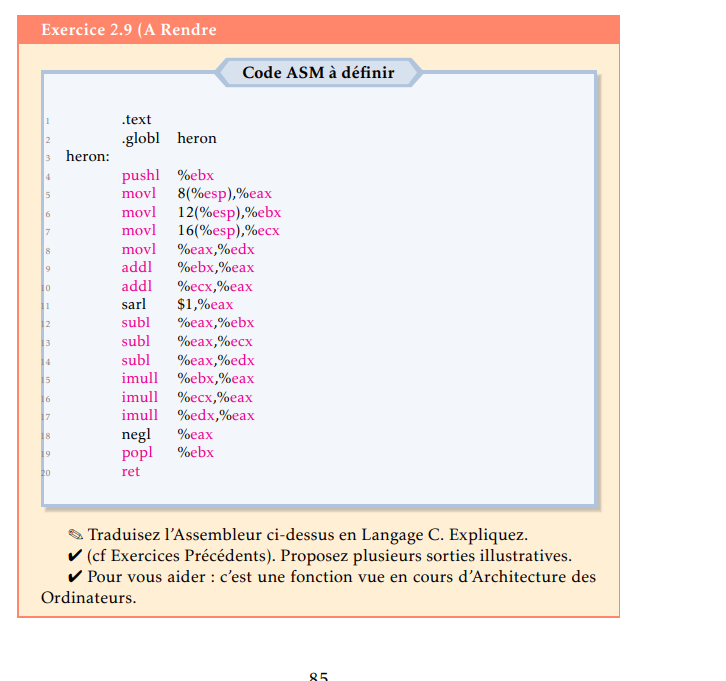
\includegraphics[width=0.85\textwidth]{images/quest2_9.png}
    \captionof{figure}{Exercice 2.9}
    \label{fig:exo2_9}
\end{center}

\subsection{Développement}
Ce code assembleur implémente la formule géométrique de Héron pour calculer l’aire d’un triangle à partir de ses trois côtés. Voici la traduction en C, expliquée ligne par ligne :

\begin{figure}[!ht]
    \centering
    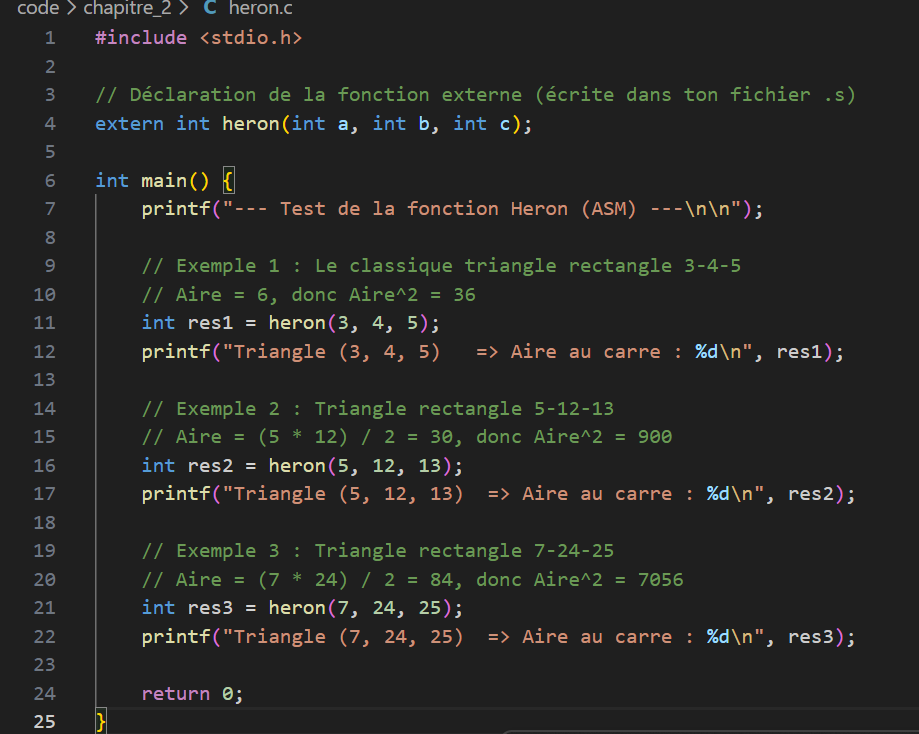
\includegraphics[width=0.85\textwidth]{images/heron_c.png} 
    \caption{Traduction en C de l'exercice 2.9}
    \label{fig:code_exo2_9_c}
\end{figure}
\begin{figure}[!ht]
    \centering
    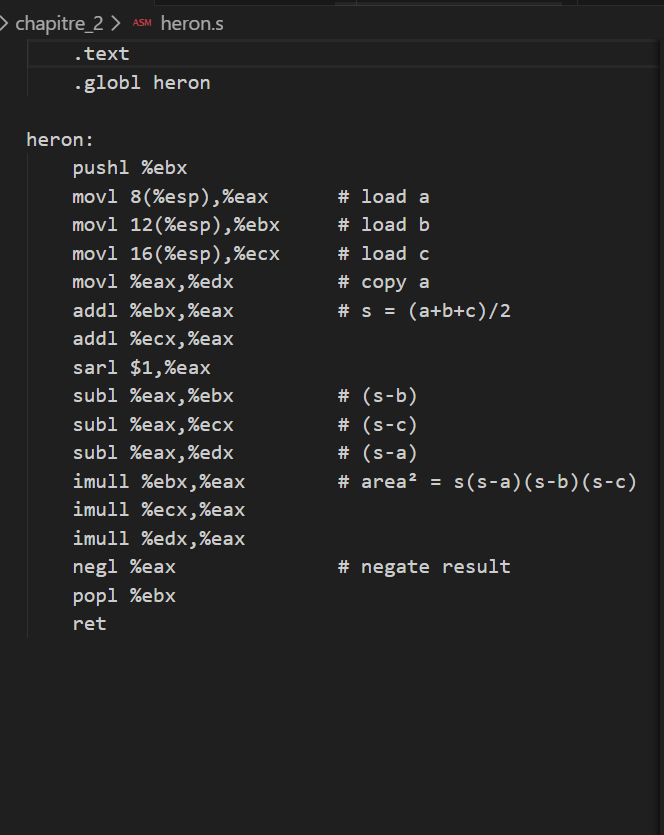
\includegraphics[width=0.85\textwidth]{images/heron_assem.png} 
    \caption{Code assembleur de l'exercice 2.9}
    \label{fig:code_exo2_9_assem}
\end{figure}

\subsubsection*{Réponse et analyse des résultats}
\paragraph*{Interprétation :}
L'exercice démontre la capacité de l'assembleur à manipuler des structures de calcul simples et des opérations arithmétiques pour répondre à des besoins mathématiques. Il souligne l'importance de la gestion des registres "callee-saved" (comme \texttt{\%ebx}) pour garantir que l'appel depuis le langage C ne provoque pas d'instabilité système. L'utilisation de \texttt{negl} et de \texttt{sarl} montre également comment l'assembleur optimise les opérations mathématiques (négation et division par deux) au niveau du processeur.

\subsubsection*{Compilation et exécution}   

Pour compiler et exécuter le programme, nous utilisons les commandes suivantes :

\begin{verbatim}
 gcc -m32 -o heron_test  heron.c heron.s
./heron_test
\end{verbatim}

\begin{figure}[!ht]
    \centering
    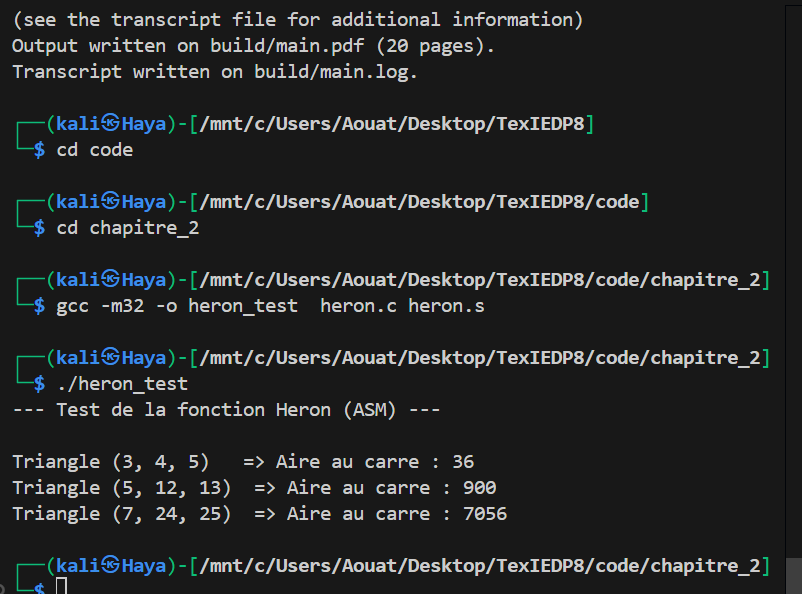
\includegraphics[width=0.85\textwidth]{images/res2.9.png} 
    \caption{Résultat de l'exécution du programme}
    \label{fig:resultat_exec_heron}
\end{figure}

\chapter{Comprendre un programme compilé en C}

\section*{Introduction}

Pour ce troisième chapitre, vous devez rendre trois exercices au choix. L'exercice 3.6 est un Bonus ou un Super Bonus.


\section{Exercice 3.1 (A choix (obligé))}
\subsection{Question}
Examinez le code produit par le compilateur quand il compile la fonction suivante :

\begin{verbatim}
void foo() {
    if (0 == 1)
        printf("Hello\n"); // jamais exécuté
}
\end{verbatim}

En faisant varier le niveau d'optimisation de la compilation sous GCC, l'appel à la fonction \texttt{printf} est-il encore dans le code ?

Et la chaîne de caractère \texttt{"Hello"} ?

\textbf{Note :} N'oubliez pas d'insérer les copies d'écran (ou textuelles) commentées avec les lignes de compilation. Pour plus de lisibilité, vous pouvez surligner les parties intéressantes du code produit.

\subsection{Développement}
Pour observer l'effet des optimisations, le même code C est compilé en assembleur avec deux niveaux : sans optimisation (\texttt{-O0}) et avec optimisation (\texttt{-O2}).

\begin{verbatim}
gcc -O0 -S foo.c -o foo_O0.s
gcc -O2 -S foo.c -o foo_O2.s
\end{verbatim}

Le code source utilisé est illustré ci-dessous :

\begin{figure}[!ht]
    \centering
    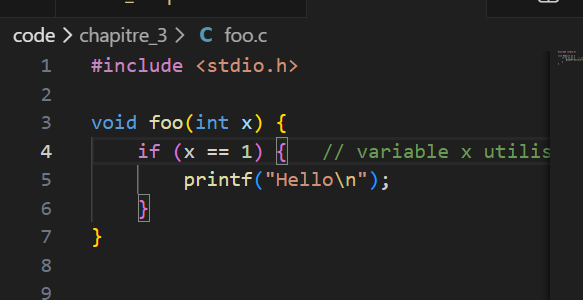
\includegraphics[width=0.85\textwidth]{images/foo_c.png}
    \caption{Code source de foo.c}
    \label{fig:code_foo_c}
\end{figure}

Les deux assemblages générés sont comparés ci-après :

\begin{figure}[!ht]
    \centering
    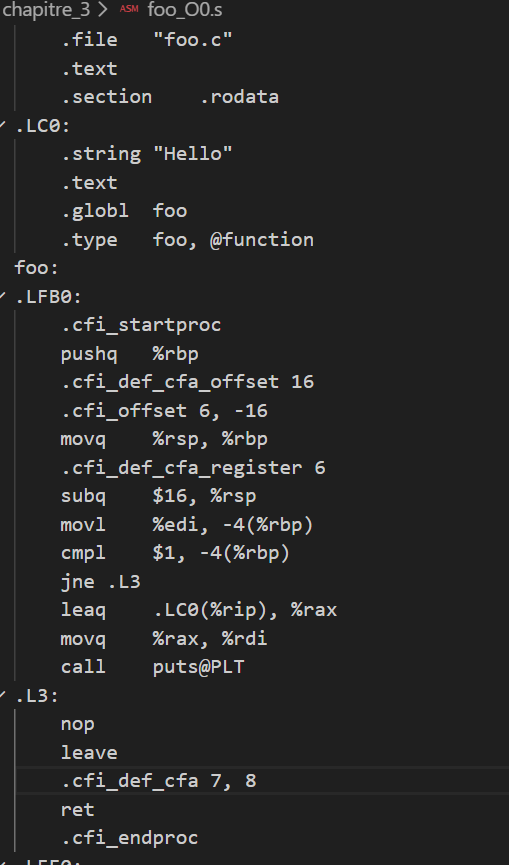
\includegraphics[width=0.85\textwidth]{images/foo_assemb.png}
    \caption{Assemblage obtenu avec \texttt{-O0} et \texttt{-O2}}
    \label{fig:code_foo_asm}
\end{figure}

\subsubsection*{Analyse des résultats}
\begin{itemize}
    \item \textbf{-O0 (sans optimisation)} : le code contient l'appel à \texttt{printf} et la chaîne \texttt{"Hello"} car le compilateur ne supprime pas le code mort.
    \item \textbf{-O2 (optimisé)} : l'appel à \texttt{printf} et la chaîne \texttt{"Hello"} sont supprimés si la condition est constante (\texttt{if (0 == 1)}), car le bloc est évalué comme inatteignable.
    \item \textbf{Comportement attendu} : pour conserver le code dans la version optimisée, il faut empêcher le compilateur de prouver que le test est toujours faux (par exemple en utilisant une variable lue à l'exécution).
\end{itemize}

\subsection{Analyse}
L'exercice illustre comment les optimisations du compilateur peuvent éliminer le code mort, améliorant ainsi l'efficacité du programme final. Il souligne l'importance de comprendre le comportement du compilateur pour éviter des suppressions inattendues de code, en particulier dans des contextes où certaines branches doivent être conservées pour des raisons logiques ou de débogage.
Donc finalement, avec l'optimisation activée, l'appel à \texttt{printf} et la chaîne \texttt{"Hello"} ne sont plus présents dans le code compilé.

\subsection{Exercice 3.2 (Au choix - À rendre)}

\subsection{Question}
Examinez le code produit par le compilateur quand il compile la fonction suivante :

\begin{verbatim}
void foo(int x) {
    if (x == x + 1)
        printf("Hello\n"); // jamais exécuté
}
\end{verbatim}

Avec les mêmes consignes que l'exercice précédent en ce qui concerne les variations d'optimisation de la compilation sous GCC, l'appel à la fonction \texttt{printf} est-il encore dans le code ?

Et aussi la chaîne de caractère \texttt{"Hello"} ?

\textbf{Note :} N'oubliez pas d'insérer les copies d'écran (ou textuelles) commentées avec les lignes de compilation. Pour plus de lisibilité, vous pouvez surligner les parties intéressantes du code produit.

\subsection{Développement}
Cette variante introduit une condition symbolique : \texttt{if (x == x + 1)}. Contrairement au cas précédent, la valeur de \texttt{x} n'est pas connue à l'avance, mais la relation logique est mathématiquement impossible pour tout entier.

Voici les commandes pour compiler en assembleur :

\begin{verbatim}
gcc -O0 -S foo_sec.c -o foo_sec_O0.s
gcc -O2 -S foo_sec.c -o foo_sec_O2.s
\end{verbatim}

\begin{figure}[!ht]
    \centering
    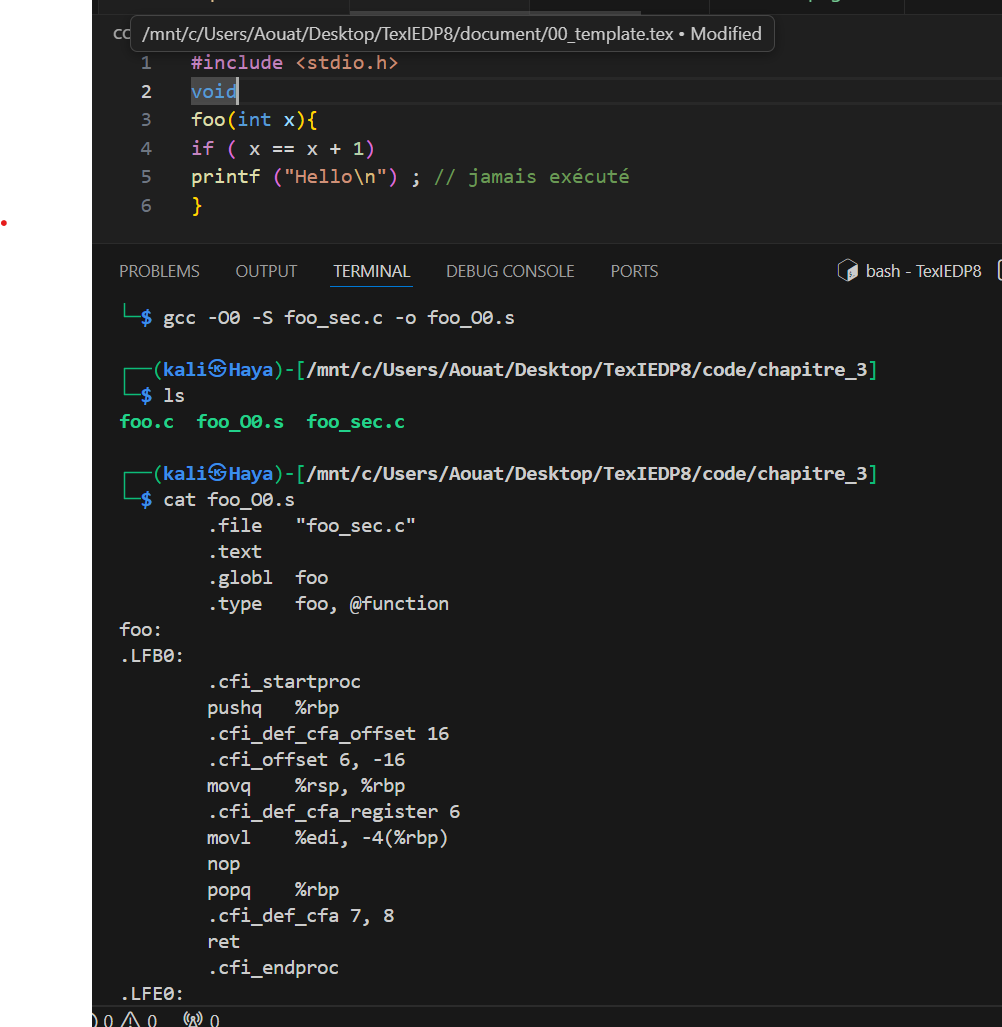
\includegraphics[width=0.85\textwidth]{images/3_2.png}
    \caption{Code source de foo\_sec.c et résultat de compilation avec \texttt{-O0}}
    \label{fig:code_foo_sec_c}
\end{figure}

Lors de nos tests avec GCC version 14.3.0, nous avons observé que même avec l'option \texttt{-O0}, le compilateur élimine le code mort de la condition \texttt{x == x + 1}. Cela s'explique par les mécanismes d'\textit{early optimization} intégrés aux compilateurs modernes. GCC identifie l'impossibilité algébrique $x = x + 1$ dès la phase d'analyse sémantique, avant même la génération du code assembleur.

\begin{figure}[!ht]
    \centering
    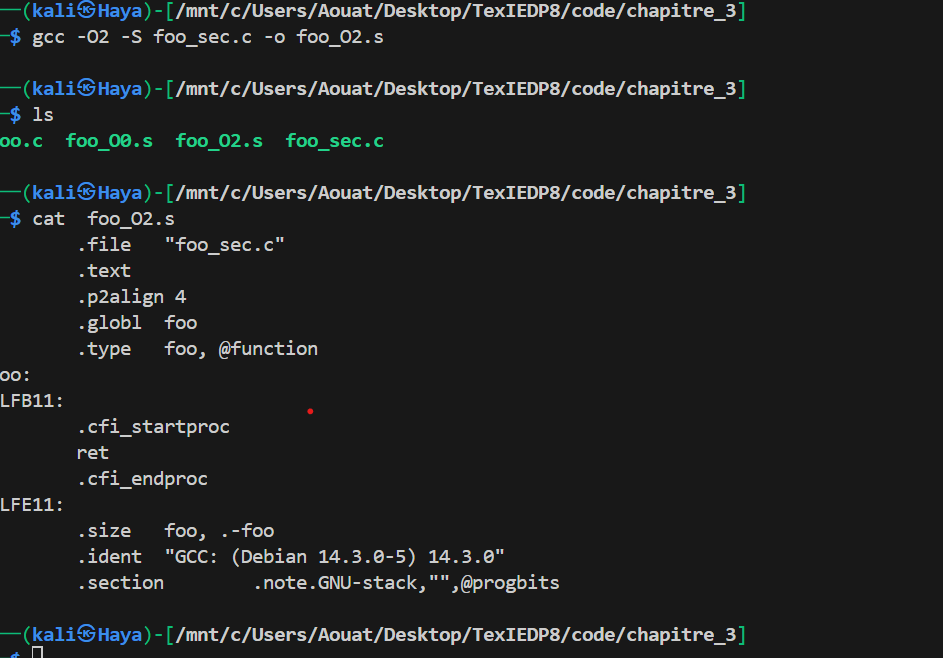
\includegraphics[width=0.85\textwidth]{images/3_2_2.png}
    \caption{Résultat de compilation avec \texttt{-O2}}
    \label{fig:code_foo_sec_O2}
\end{figure}

\subsubsection*{Analyse des résultats}

\begin{itemize}
    \item \textbf{La fonction printf est supprimée} : le compilateur, avec l'option \texttt{-O2}, analyse la logique mathématique. Il « sait » qu'un nombre entier ne peut jamais être égal à lui-même plus un ($x \neq x + 1$). Il en conclut que le bloc \texttt{printf} ne sera jamais exécuté.
    \item \textbf{Cas sans optimisation} : même avec \texttt{-O0}, le compilateur reconnaît l'absurdité mathématique et supprime le code.
    \item \textbf{Vérification dans l'assembleur} : il y a \texttt{ret} directement après l'entrée de la fonction, indiquant qu'elle se termine immédiatement sans exécuter d'autres instructions.
\end{itemize}

\subsection{Analyse}

L'examen du fichier \texttt{foo\_O2.s} révèle une fonction réduite à une seule instruction \texttt{ret}.

Contrairement au cas précédent où la condition était une constante (\texttt{0 == 1}), ici le compilateur GCC réalise une \textbf{simplification algébrique}. Il identifie que la relation $x = x + 1$ est une contradiction logique. En conséquence :

\begin{itemize}
    \item \textbf{L'appel à printf} est totalement éliminé du flux d'exécution.
    \item \textbf{La chaîne "Hello"} est supprimée des ressources du programme, n'étant plus référencée.
\end{itemize}

Ce résultat confirme que l'optimisation \texttt{-O2} ne se limite pas à accélérer le code existant, mais nettoie intelligemment le programme de toute branche .

\section{Exercices 3.3 (Au choix - À rendre)}
\subsection{Question}
La fonction snowWhite ci-dessous n’a pas besoin d’avoir sept arguments pour mettre la particularité de GCC en évidence :
 Quel est le nombre minimum d’arguments pour apercevoir
cette particularité ?
✎ S’il n’y a que deux arguments, où sont-ils placés ?
✎ S’il n’y a qu’un seul argument, où est-il placé ?
✔ (Idem que pour les exercices précédents). Evitez de plus d’utiliser l’optimisation de GCC qui risque rendre la lecture moins aisée.
Et pour plus de lisibilité, vous pouvez, comme à l’habitude, surligner les parties intéressantes du code produit.

\subsection{Développement}
La fonction \texttt{snowWhite} est conçue pour démontrer comment GCC gère

Voici la commande de compilation utilisée pour générer le code assembleur sans optimisations :
\begin{verbatim}
    gcc -O0 -S snow.c -o snow.s
cat snow.s
\end{verbatim}
Voici la résultat:
\begin{figure}[!ht]
    \centering
    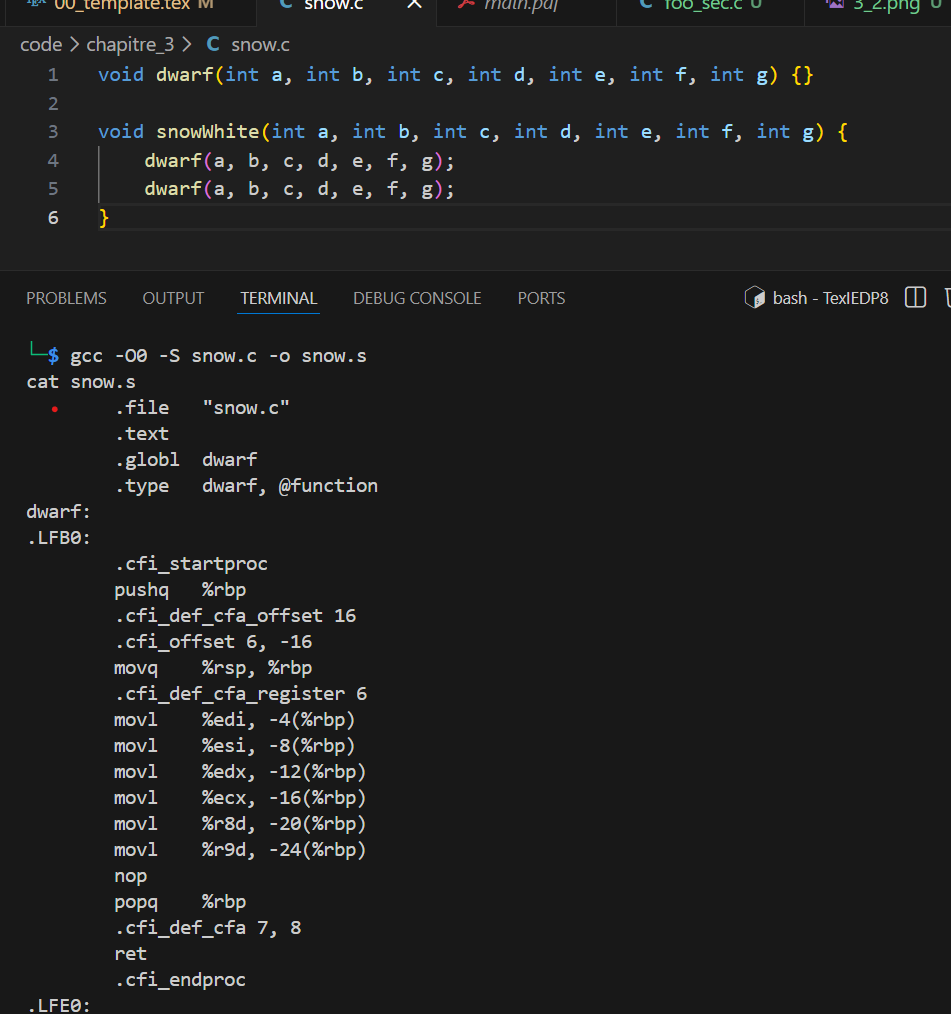
\includegraphics[width=0.85\textwidth]{images/terminal3_6.png} 
    \caption{Code assembleur généré pour snowWhite commande cli}
    \label{fig:code_snow_assem}
\end{figure}
\begin{figure}[!ht]
    \centering
    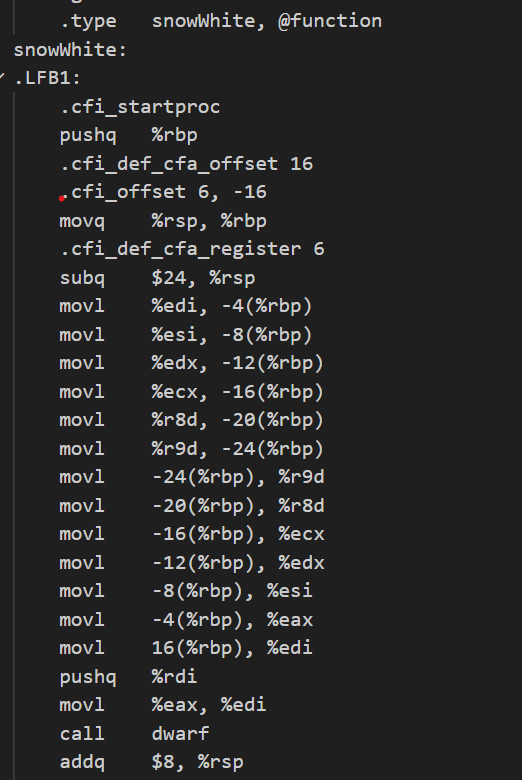
\includegraphics[width=0.85\textwidth]{images/snow_assemb.png} 
    \caption{Code assembleur généré pour snowWhite}
    \label{fig:code_snow_assem2}
\end{figure}
\subsubsection*{Analyse des résultats}

\subsection{Analyse de l'assemblage}
L'examen du fichier \texttt{snow.s} permet d'identifier deux mécanismes distincts pour le passage des paramètres :

\begin{itemize}
    \item \textbf{Par registres} : Les six premiers arguments sont reçus et manipulés via les registres dédiés de l'architecture 64 bits.
    \item \textbf{Par la pile} : À partir du septième argument, le compilateur utilise la mémoire (pile).
\end{itemize}

\begin{lstlisting}[language={[x86masm]Assembler}, caption=Passage des paramètres dans snowWhite, escapeinside={(*}{*)}]
# --- LES 6 PREMIERS ARGUMENTS (PASSES PAR REGISTRES) ---
movl    %edi, -4(%rbp)   # 1er arg (a) recu dans %edi
movl    %esi, -8(%rbp)   # 2eme arg (b) recu dans %esi
movl    %edx, -12(%rbp)  # 3eme arg (c) recu dans %edx
movl    %ecx, -16(%rbp)  # 4eme arg (d) recu dans %ecx
movl    %r8d, -20(%rbp)  # 5eme arg (e) recu dans %r8d
movl    %r9d, -24(%rbp)  # 6eme arg (f) recu dans %r9d

# --- LA PARTICULARITE : LE 7eme ARGUMENT (PILE) ---
movl    16(%rbp), %edi   # Recupere 'g' (deja sur la pile a +16)
pushq   %rdi             # (*\textbf{POUSSE 'g' sur la pile pour l'appel dwarf}*)
                         # C'est l'argument minimum pour voir ca !

movl    %eax, %edi       # Prepare 'a' pour l'appel
call    dwarf            # Appel de la fonction
addq    $8, %rsp         # Nettoie la pile (retire le 7eme argument)
\end{lstlisting}

\subsection{Réponses aux questions}

\paragraph{Quel est le nombre minimum d’arguments pour apercevoir cette particularité ?}
Le nombre minimum est \textbf{7}. Comme le démontre le code produit, GCC utilise les 6 registres standards (\texttt{\%edi} à \texttt{\%r9d}) conformément à l'ABI System V. Le 7ème argument ne peut plus être stocké dans un registre de paramètre et force l'utilisation de la pile mémoire via l'instruction \texttt{pushq}.

\paragraph{S’il n’y a que deux arguments, où sont-ils placés ?}
Ils sont placés exclusivement dans les deux premiers registres de la convention :
\begin{itemize}
    \item \texttt{\%edi} pour le premier argument.
    \item \texttt{\%esi} pour le second argument.
\end{itemize}

\paragraph{S’il n’y a qu’un seul argument, où est-il placé ?}
Il est placé uniquement dans le registre \textbf{\texttt{\%edi}}.

\paragraph{Interprétation :}
Cette observation confirme que l'architecture x86-64 optimise les appels de fonction en utilisant les registres (plus rapides) pour les six premiers arguments entiers, et ne sollicite la mémoire (pile) que lorsque ce quota est dépassé.

\chapter{L'analyse lexicale et syntaxique}
\section*{Introduction}
Pour ce quatrième chapitre, vous devez rendre les exercices 4.3 et 4.11, ainsi que deux exercices au choix (l’un dans la première série d’exercices et l’autre dans la seconde), les difficultés étant variables. Les exercices au choix 4.17 et 4.18 sont pour un Bonus.

\section{Exercice 4.3 (À rendre)}
\subsection{Question}
Modifiez le programme \texttt{dc-elem.c} pour pouvoir effectuer les autres opérations arithmétiques usuelles (soustraction, multiplication, division et modulo). Expliquez.

\textbf{Note :} Commentez les lignes ajoutées et produisez deux ou trois sorties illustratives du programme modifié.

\subsection{Développement}
L'objectif de cet exercie est de pouvoir rajouté les opérateurs arithmétiques du langage C
Nous avons modifié le fichier \texttt{dc-elem\_all.c} en intervenant sur trois points clés :
\begin{itemize}
    \item \textbf{L'analyseur lexical (\texttt{yylex})} : Ajout des caractères \texttt{'-', '*', '/', '\%'} dans la condition de détection des terminaux.
    \item \textbf{L'analyseur syntaxique (\texttt{yyparse})} : Mise à jour de la vérification de l'opérateur pour accepter ces nouveaux jetons.
    \item \textbf{L'unité de calcul} : Implémentation d'une structure \texttt{if...else if} pour exécuter l'opération correspondante, incluant une sécurité pour la division par zéro.
\end{itemize}



Voici les commandes pour compiler et tester le programme sous Kali Linux :

\begin{verbatim}
gcc dc-elem_all.c -o dc-elem_all
./dc-elem_all
\end{verbatim}

\begin{figure}[!ht]
    \centering
    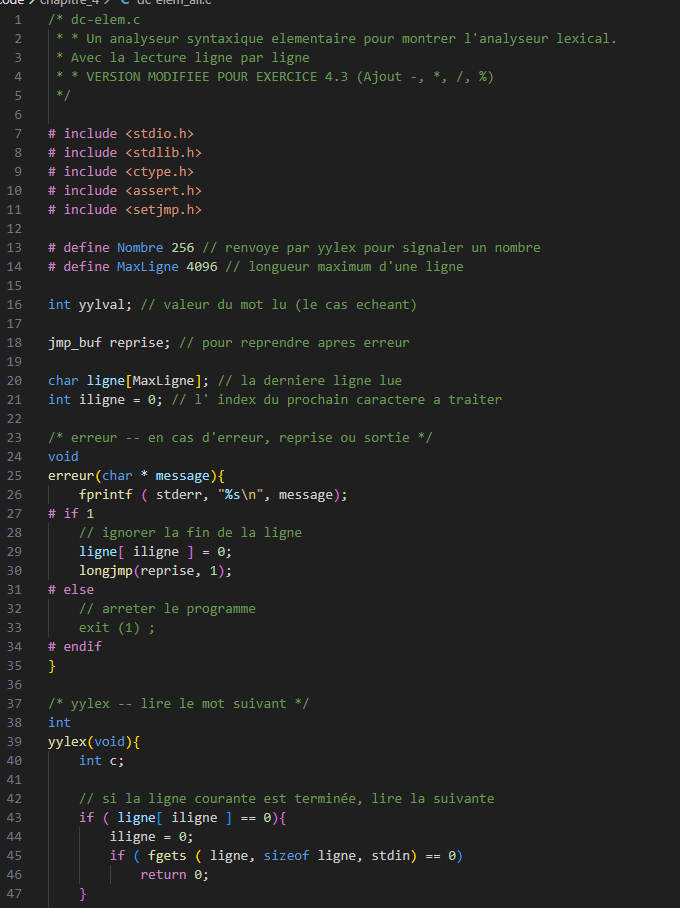
\includegraphics[width=0.85\textwidth]{images/chap4/1.png}
    \caption{Modifications apportées au code source de \texttt{dc-elem\_all.c}}
    \label{fig:code_modifie}
\end{figure}
\begin{figure}[!ht]
    \centering
    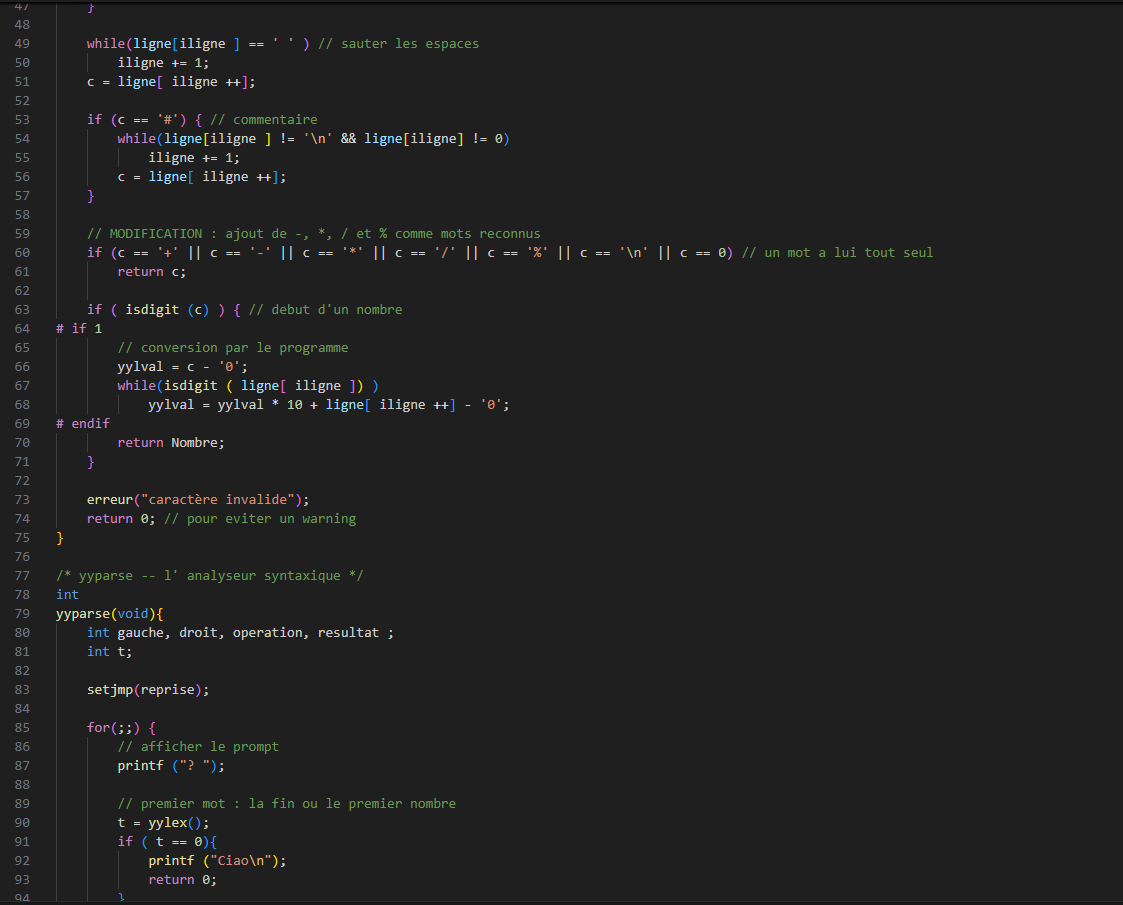
\includegraphics[width=0.85\textwidth]{images/chap4/2.png}
    \caption{Modifications apportées au code source de \texttt{dc-elem\_all.c}}
    \label{fig:code_modifie}
\end{figure}
\begin{figure}[!ht]
    \centering
    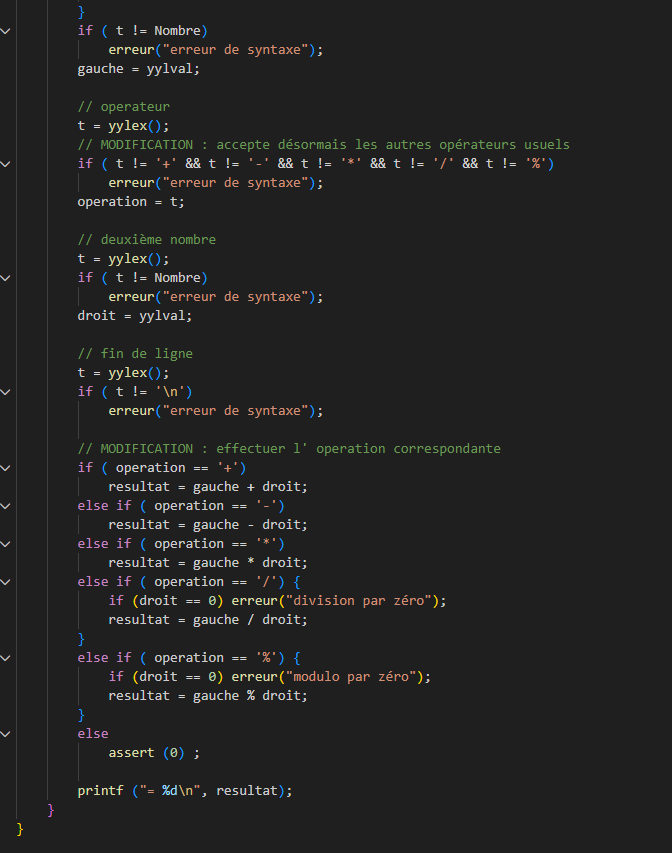
\includegraphics[width=0.85\textwidth]{images/chap4/3.png}
    \caption{Modifications apportées au code source de \texttt{dc-elem\_all.c}}
    \label{fig:code_modifie}
\end{figure}
\begin{figure}[!ht]
    \centering
    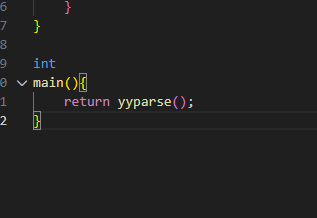
\includegraphics[width=0.85\textwidth]{images/chap4/4.png}
    \caption{Modifications apportées au code source de \texttt{dc-elem\_all.c}}
    \label{fig:code_modifie}
\end{figure}


\subsubsection*{Code source modifié}
Dans \texttt{yylex} :
\begin{verbatim}
// Ajout des nouveaux opérateurs dans les caractères reconnus
if (c == '+' || c == '-' || c == '*' || c == '/' || c == '%' || c == '\n' || c == 0)
    return c;
\end{verbatim}

Dans \texttt{yyparse} :
\begin{verbatim}
// Calcul selon l'opérateur reçu
if (operation == '+') resultat = gauche + droit;
else if (operation == '-') resultat = gauche - droit;
else if (operation == '*') resultat = gauche * droit;
else if (operation == '/') {
    if (droit == 0) erreur("division par zero");
    resultat = gauche / droit;
}
else if (operation == '%') {
    if (droit == 0) erreur("modulo par zero");
    resultat = gauche % droit;
}
\end{verbatim}

\begin{figure}[!ht]
    \centering
    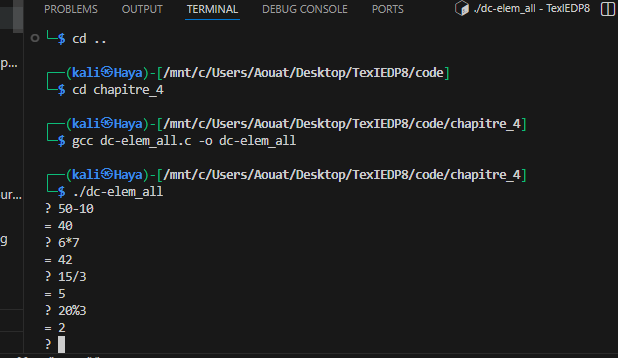
\includegraphics[width=0.85\textwidth]{images/chap4/res_3.png}
    \caption{Exécution du programme et tests des opérations (Multiplication, Division, Modulo)}
    \label{fig:tests_4_3}
\end{figure}

\subsection{Analyse des résultats}

L'examen des sorties du programme (Figure \ref{fig:tests_4_3}) confirme le bon fonctionnement de l'extension :

\begin{itemize}
    \item \textbf{Polyvalence} : Le programme traite désormais correctement les soustractions (\texttt{50-10}), multiplications (\texttt{6*7}) et divisions entières.
    \item \textbf{Le Modulo} : L'opérateur \texttt{\%} renvoie bien le reste de la division euclidienne (ex: \texttt{20 \% 3 = 2}).
    \item \textbf{Gestion des erreurs} : L'ajout d'un test sur le diviseur nul permet d'éviter un crash du système (\textit{Floating point exception}) en renvoyant une erreur explicite via la fonction \texttt{erreur} et le mécanisme de \texttt{longjmp}.
    \item \textbf{Lexique} : L'analyseur lexical ignore correctement les espaces et reconnaît les nouveaux opérateurs comme des entités syntaxiques valides.
\end{itemize}

Ce développement démontre comment une grammaire simple peut être étendue en enrichissant conjointement le dictionnaire de jetons (lexique) et les règles d'interprétation (syntaxe)


\section{Exercice 4.11 (À rendre)}
\subsection{Question}
Soit la grammaire :

\begin{verbatim}
p : A B
p : A p B
\end{verbatim}

\subsubsection*{Tâches}
\begin{itemize}
    \item Générez à partir de cette grammaire des phrases de 2, 4, 6 et 8 mots.
    \item Écrivez en une phrase le langage décrit par cette grammaire.
    \item (Plus difficile) Trouvez une expression régulière pour le langage décrit par cette grammaire, ou expliquez pourquoi ce n’est pas possible.
\end{itemize}

\textbf{Note :} Dessinez l’arbre syntaxique avec le logiciel de votre choix et explicitez vos réponses.

\subsection{Développement}
Cette grammaire est récursive. Le symbole non-terminal \texttt{p} peut se dériver soit en une paire terminale \texttt{A B}, soit s'étendre en entourant un nouveau \texttt{p} par un \texttt{A} à gauche et un \texttt{B} à droite.

\subsubsection*{Génération de phrases}
En appliquant les règles de dérivation, nous obtenons :
\begin{itemize}
    \item \textbf{2 mots} : $p \rightarrow A B$
    \item \textbf{4 mots} : $p \rightarrow A p B \rightarrow A (A B) B \rightarrow A A B B$
    \item \textbf{6 mots} : $p \rightarrow A p B \rightarrow A (A p B) B \rightarrow A A (A B) B B \rightarrow A A A B B B$
    \item \textbf{8 mots} : $p \rightarrow A p B \rightarrow A A A p B B B \rightarrow A A A A B B B B$
\end{itemize}

\begin{figure}[!ht]
    \centering
    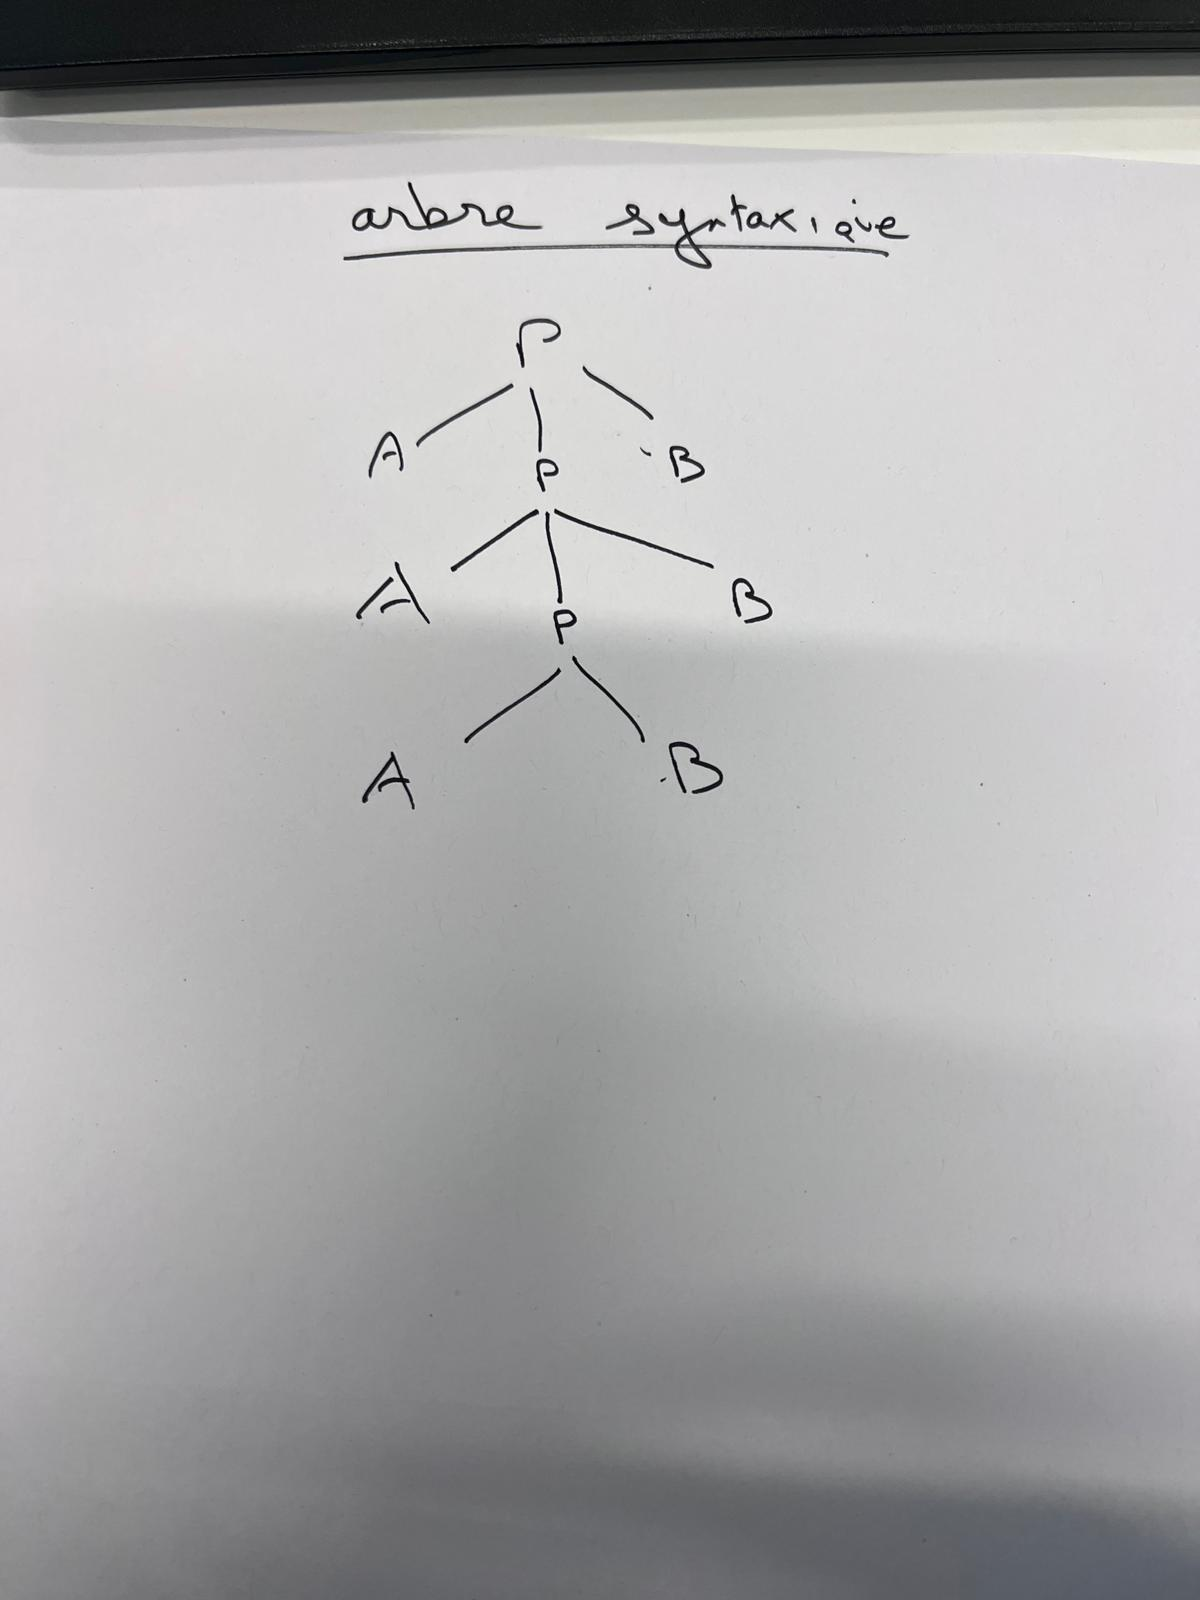
\includegraphics[width=0.6\textwidth]{images/chap4/shema.jpeg}
    \caption{Arbre syntaxique pour la phrase "AAABBB" (6 mots)}
    \label{fig:arbre_syntaxique}
\end{figure}

\subsubsection*{Définition du langage}
Le langage décrit par cette grammaire est l'ensemble des mots commençant par un certain nombre de symboles \texttt{A} suivis du \textbf{même nombre} de symboles \texttt{B}. On peut le noter mathématiquement : $L = \{A^n B^n \mid n \geq 1\}$.

\subsection{Analyse des résultats}

\subsubsection*{Expression régulière}
Il est **impossible** de trouver une expression régulière pour ce langage.

\textbf{Pourquoi ?} 
Une expression régulière ne peut pas "compter" ou mémoriser un nombre indéfini de caractères. Ici, le langage impose d'avoir **exactement** le même nombre de \texttt{A} et de \texttt{B} ($A^n B^n$). 

\textbf{Conclusion :} 
Comme un automate fini (utilisé par les expressions régulières) a une mémoire limitée, il ne peut pas vérifier que le compteur de \texttt{A} est égal au compteur de \texttt{B}. C'est pour cela qu'on utilise une \textbf{grammaire hors-contexte} (avec une pile) plutôt qu'une simple expression régulière.


\subsection{Exercice 4.12 (Au choix — À rendre)}
\subsection{Question}
Avec la grammaire ci-dessous :

\begin{verbatim}
p : /* rien */
p : A p B p
\end{verbatim}

\subsubsection*{Tâches}
\begin{itemize}
    \item (Idem) Générez à partir de cette grammaire toutes les phrases de 2 mots, de 4 mots, de 6 mots.
\end{itemize}
La grammaire est un peu plus "libre" que la précédente. Elle permet non seulement d'imbriquer les lettres (les unes dans les autres), mais aussi de les mettre les unes après les autres (juxtaposition). C'est le principe des parenthèses bien formées : chaque \texttt{A} ouvert doit être fermé par un \texttt{B}.

\subsubsection*{Génération des phrases}

En remplaçant les \texttt{p} soit par "rien", soit par la règle \texttt{A p B p}, on obtient :

\begin{itemize}
    \item \textbf{2 mots (1 seule possibilité)} :
    \begin{itemize}
        \item \textbf{AB} (on a remplacé les deux \texttt{p} par rien).
    \end{itemize}

    \item \textbf{4 mots (2 possibilités)} :
    \begin{itemize}
        \item \textbf{AABB} (on a mis un bloc à l'intérieur).
        \item \textbf{ABAB} (on a mis deux blocs à la suite).
    \end{itemize}

    \item \textbf{6 mots (5 possibilités)} :
    \begin{itemize}
        \item \textbf{AAABBB} (tout est imbriqué).
        \item \textbf{AABABB} (un bloc suivi d'un petit, le tout dans un grand).
        \item \textbf{AABBAA} (impossible ici, car l'ordre impose \texttt{B} après \texttt{A}).
        \item En réalité, on trouve : \textbf{AAABBB}, \textbf{AABABB}, \textbf{ABAABB}, \textbf{AABBAB} et \textbf{ABABAB}. 
    \end{itemize}
\end{itemize}

\subsection{Analyse des résultats}

La grosse différence avec l'exercice d'avant, c'est que le \texttt{p} à la fin de la règle (\texttt{A p B \textbf{p}}) permet de recommencer une séquence après avoir fermé la première. C'est pour ça qu'on peut avoir des phrases comme \texttt{ABAB}. 
Finalement cette grammaire génère tous les schémas de parenthèses qui se ferment correctement. Plus on augmente le nombre de mots, plus il y a de combinaisons possibles

\chapter{Utilisation du compilateur Yacc}
\section*{Introduction}
Pour ce cinquième chapitre sur Yacc et Bison, vous devez rendre les exercices 5.2 et 5.3 et un exercice au choix parmi les deux présentés. L’exercice
5.6 est pour un Bonus.

\section {Exercice 5.2 (A rendre)}
\subsection{Question}
Modifiez la fonction \texttt{parenthese} (cf. code \texttt{1-calc.y}) pour qu’elle n’imprime que les parenthèses nécessaires. Expliquez votre démarche.

\paragraph{Exemples attendus :}
\begin{verbatim}
(1)             -> 1
((1))           -> 1
(1 + (2 + 3))   -> 1 + 2 + 3
((1 + 2) + 3)   -> 1 + 2 + 3
1 + (2 * 3)     -> 1 + 2 * 3
1 * (2 + 3)     -> 1 * (2 + 3)
\end{verbatim}

\subsection{Développement}  
Pour résoudre cet exercice et gérer l'affichage intelligent des parenthèses, nous avons dû passer d'une évaluation directe (calcul immédiat) à une approche basée sur un \textbf{Arbre de Syntaxe Abstraite (AST)}. 

En effet, pour savoir si une parenthèse est nécessaire, il ne suffit pas de connaître la valeur d'une sous-expression, il faut connaître sa structure et l'opérateur qui la lie à son parent. L'AST permet de conserver cette hiérarchie. Chaque nœud de l'arbre représente soit un nombre, soit un opérateur avec ses deux fils (gauche et droit). 


\subsection{Compilation et Exécution}
\begin{verbatim}
    On lance le code avec gcc 1-calc-reecriture.c -o 1-calc-reecriture
    puis: ./1-calc-reecriture
\end{verbatim}
\begin{figure}[!ht]
    \centering
    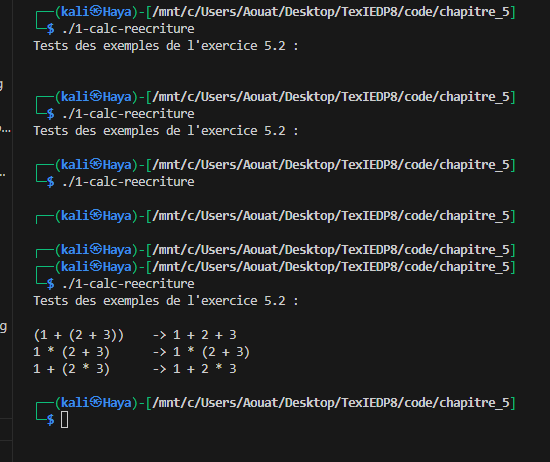
\includegraphics[width=0.6\textwidth]{images/chap5/cmdcompilation.png}
    \caption{Extrait du code source de la commande de compilation}
    \label{fig:cmdcompilation}
\end{figure}


\section{Code et Explications}
\begin{figure}[!ht]
    \centering
    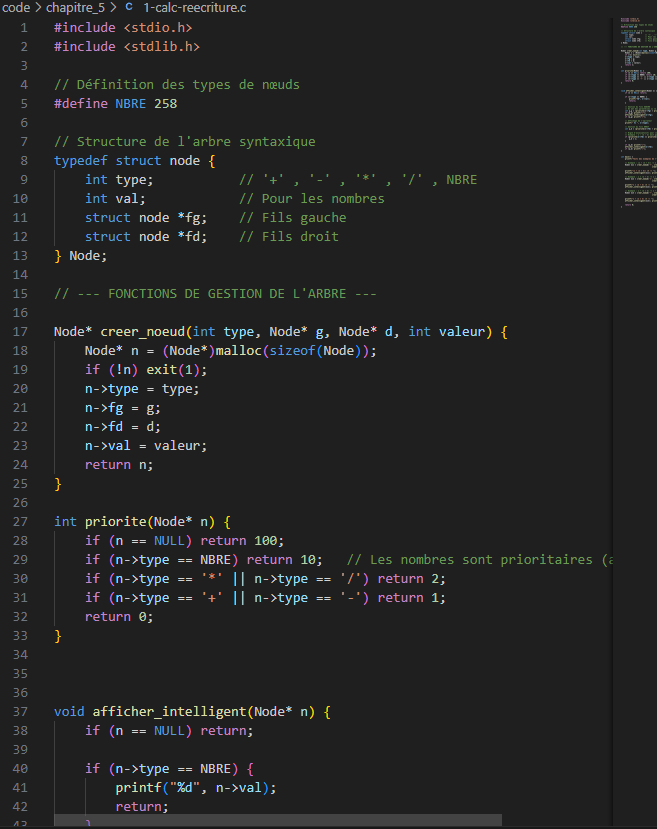
\includegraphics[width=0.6\textwidth]{images/chap5/image1.png}
    \caption{Extrait du code source de 1-calc-reecriture.c}
    \label{fig:code_1-calc-reecriture}
\end{figure}

\begin{figure}[!ht]
    \centering
    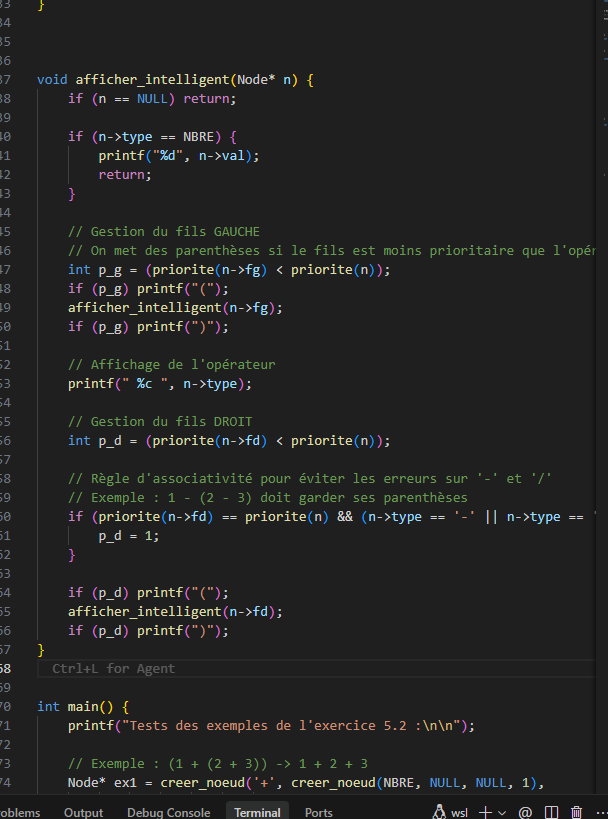
\includegraphics[width=0.6\textwidth]{images/chap5/image2.png}
    \caption{Extrait du code source de 1-calc-reecriture.c}
    \label{fig:code_1-calc-reecriture}
\end{figure}

\begin{figure}[!ht]
    \centering
    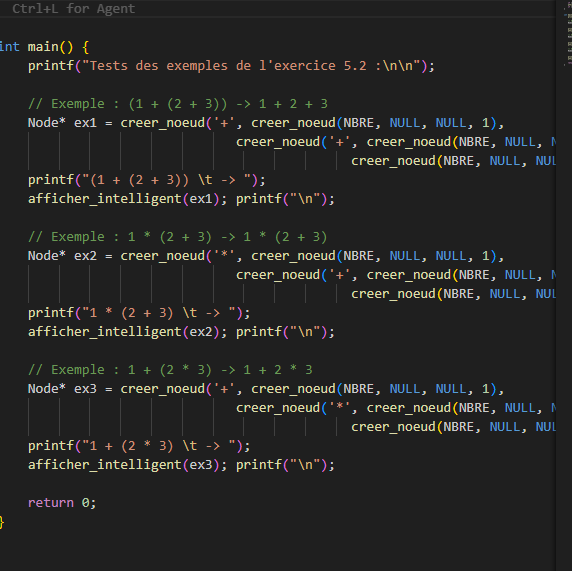
\includegraphics[width=0.6\textwidth]{images/chap5/image3.png}
    \caption{Extrait du code source de 1-calc-reecriture.c}
    \label{fig:code_1-calc-reecriture}
\end{figure}

\subsection{Explications}
L'algorithme de réécriture repose sur la comparaison des priorités entre un nœud parent et ses nœuds fils lors d'un parcours récursif de l'arbre.

\begin{itemize}
    \item \textbf{Gestion des priorités :} Nous avons défini une fonction \texttt{priorite()} qui attribue une valeur numérique à chaque opérateur (ex: 2 pour \texttt{*} et \texttt{/}, 1 pour \texttt{+} et \texttt{-}). 
    \item \textbf{Parcours récursif :} La fonction \texttt{afficher\_intelligent()} parcourt l'arbre. Pour chaque nœud, elle vérifie si la priorité du fils est inférieure à celle du parent. Si c'est le cas, elle entoure l'affichage du fils par des parenthèses.
    \item \textbf{Cas particulier de l'associativité :} Pour les opérateurs comme la soustraction (\texttt{-}) et la division (\texttt{/}), l'ordre des opérations est crucial. Par exemple, $1 - (2 - 3)$ n'est pas égal à $1 - 2 - 3$. L'algorithme détecte si le fils droit a la même priorité que le parent pour ces opérateurs spécifiques et impose des parenthèses afin d'éviter une modification du sens mathématique de l'expression.
\end{itemize}

\subsection{Conclusion}
L'implémentation de cet affichage "intelligent" démontre l'importance de l'AST dans la conception d'un compilateur. Au-delà du simple calcul, la structure en arbre permet d'effectuer des transformations symboliques et de la réécriture de code. Cette technique est à la base des outils de "pretty-printing" et de refactorisation automatique, où l'on cherche à produire un code source à la fois correct syntaxiquement et lisible pour l'humain.

\section{Exercice 5.3 (A rendre)}
\subsection{Question}
\begin{figure}[!ht]
    \centering
    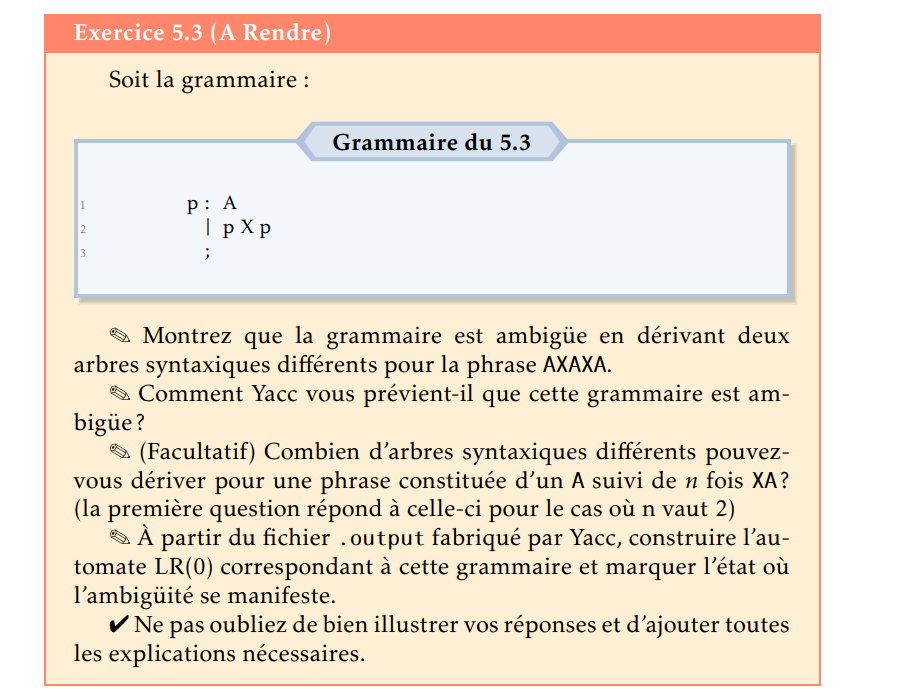
\includegraphics[width=0.6\textwidth]{images/chap5/quest5-4.png}
    \caption{consignes de l'exercice 5.4}
    \label{fig:consignes_5-4}
\end{figure}



\section{Exercice 5.5 (Au choix — À rendre)}
\subsection{Question}
\begin{figure}[!ht]
    \centering
    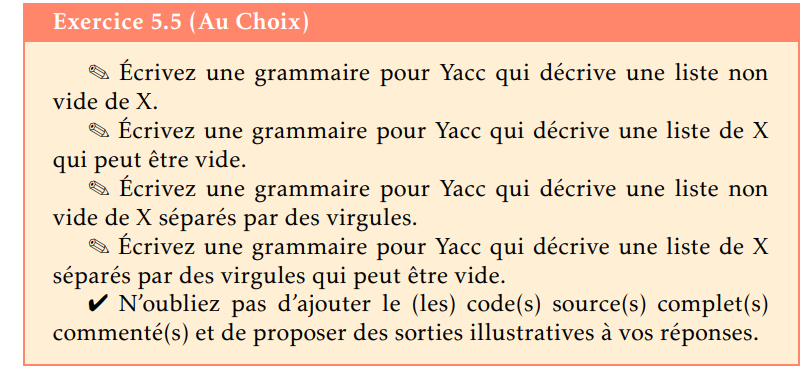
\includegraphics[width=0.6\textwidth]{images/chap5/quest5-5.png}
    \caption{consignes de l'exercice 5.5}
    \label{fig:consignes_5-5}
\end{figure}
